\documentclass[./00PhotoBox.tex]{subfiles}
\graphicspath{{\subfix{./img/}}}
\begin{document}

\chapter{Untersuchungen zur Genauigkeit und Systemaufbau}
Nach Abschluss der Konstruktion und des Aufbaus des Prototyps, wurden verschiedene Untersuchungen durchgeführt, um die Genauigkeit des Systems zu überprüfen und die Anzahl der Kameras zu evaluieren. Hierzu wurden unter anderem Vergleichsmessungen mit verschiedenen Systemen durchgeführt.

\section{Genauigkeitsüberprüfung des 3D-Modelles}
\label{s:genauigkeitsueberpruefung}
Um die Genauigkeit der 3D-Modell-Erzeugung zu überprüfen, wurden mehrere Prüf\-körper mit dem Prototyp und im Folgenden einem kommerziellen Streifenprojektionssystem vermessen. Die Ergebnisse wurden miteinander verglichen.

\subsection{Erwartete Genauigkeit}
\label{ss:erwartete_genauigkeit}
Die erwartete Genauigkeit kann auf verschiedenen Wegen berechnet werden. Grundlage ist meistens der Bildmaßstab. Dieser unterscheidet sich je nach Entfernung. Die Entfernung zum Objekt beträgt im Normalfall zwischen 10 und 50~cm. Der Bildmaßstab $m$ berechnet sich nach \cite[S. 171]{luhmann} wie folgt:

\begin{align}
    m       & = \frac{h}{c}                                  \\
    m_{min} & = \frac{100~\text{mm}}{4,7~\text{mm}} = 21,28  \\
    m_{max} & = \frac{500~\text{mm}}{4,7~\text{mm}} = 106,38
\end{align}
\begin{conditions}
    m & Bildmaßstab \\
    h & Abstand zur Kamera \\
    c & Kamerakonstante (hier 4,7~mm)
\end{conditions}

Für die Bildmessgenauigkeit werden verschiedene Werte in der Literatur erwähnt, sie liegen je nach Messmethode zwischen 0,05 und 3~px. Für Messung von CCCTs wird z.B. von \cite{soot2015} eine Genauigkeit von 0,1~px angegeben.
Eigene, manuelle Messungen ergaben eine Genauigkeit von etwa 1,5~px. Vereinfacht wurde mit 1~px Genauigkeit gerechnet.

\begin{align}
    dx'      & = 1~\text{px} = 0,0014~\frac{\text{mm}}{\text{px}} \cdot 12~\text{px} = 0,0014~\text{mm} \\
    dX       & = m \cdot dx'                                                                            \\
    dX_{min} & = 21,28 \cdot 0,0014~\text{mm} = 0,03~\text{mm}                                          \\
    dX_{max} & = 106,38 \cdot 0,0014~\text{mm} = 0,15~\text{mm}
\end{align}
\begin{conditions}
    dx' & Bildmessgenauigkeit \\
    dX  & Lage-Genauigkeit (Objektraum)
\end{conditions}

An diesem Wert muss dann noch der sogenannte Design-Faktor \todo{erklären} angebracht werden, dieser liegt bei Rundumverbänden zwischen 0,4 und 0,8, bei Stereoaufnahmen bei 1,5-3,0 \citep[S. 174]{luhmann}. Vereinfacht für eine grobe Abschätzung wird hier daher der Faktor weggelassen. Die erwartete Genauigkeit liegt damit deutlich unter einem Millimeter in der Lage.

\begin{align}
    s_{px; min}' & = dX_{min} \\
    s_{px; max}' & = dX_{max}
\end{align}

Die Genauigkeit der Tiefeninformationen ist von dem Verhältnis des Abstandes der Kameras zur Entfernung abhängig. Zwischen zwei Kamerareihen sind etwa 25~cm Abstand. Die Genauigkeit der Tiefeninformationen kann daher wie folgt berechnet werden \citep[S. 174]{luhmann}:

\begin{align}
    s_Z       & = m \cdot \frac{h}{b} \cdot s_{px}'                                                    \\
    s_{Z;min} & = 21,28 \cdot \frac{10~\text{cm}}{30~\text{cm}}\cdot 0,03~\text{mm}  = 0,02~\text{mm}  \\
    s_{Z;max} & = 106,38 \cdot \frac{50~\text{cm}}{30~\text{cm}} \cdot 0,15~\text{mm} = 0,25~\text{mm}
\end{align}
\begin{conditions}
    s_Z & Genauigkeit der Tiefeninformationen \\
    b   & Basislinie (hier 30~cm)
\end{conditions}

Die erwartete Genauigkeit und auch die Auflösung der Kameras liegt demnach im Bereich eines Fünftel Millimeters.


\subsection{Vergleichsmessung mit Streifenprojektionssystem}
Als Vergleichsmessung wurden die Objekte mit einem Zeiss GOM ATOS 5 aufgenommen. Hierbei handelt es sich um ein Streifenprojektionssystem, welches hauptsächlich in der Industrie zur Vermessung von Bauteilen eingesetzt wird. Streifenprojektionssysteme arbeiten auch photogrammetrisch, haben aber den Vorteil, das sie durch das Projektionssystem auch texturarme Objekte erfassen können. Wie der Name bereits andeutet, wird ein Streifenmuster auf das Objekt projiziert, welches dann von mindestens einer Kamera aufgenommen wird. Projektor und Kamera sind auf einer festen Basis montiert. \citep[S. 581f]{luhmann}

Bei dem verwendeten System werden zwei Kameras eingesetzt, die sich ein massives Gehäuse mit dem mittig angeordneten Projektor teilen. Bei dem verwendeten Messvolumen und Objektentfernung beträgt die Genauigkeit etwa \todo{Wert}. Aufgrund der deutlich höheren erwarteten Genauigkeit des Streifenprojektionssystems, kann davon ausgegangen werden, dass die Messungen deutlich genauer sind als die des Prototyps und als wahre Werte angenommen werden können.

\subsection{Ergebnisse}
Die modellierte Oberfläche aus dem Streifenprojektionssystem und die Punktwolke aus dem Prototyp wurden in CloudCompare aufeinandergelegt und die Differenz berechnet. Die Visualisierung der Differenzen ist in \autoref{img:differenz_moai} dargestellt. Es ist zu erkennen, dass einige Bereiche gar nicht erfasst bzw. deren Genauigkeit deutlich von der erwarteten abweichen. Die größten Fehlstellen sind im Bereich des Kinnes und unterhalb des Bauches zu erkennen. Abweichungen im Bereich des restlichen Körpers sind deutlich geringer und liegen im Bereich von 0,21~mm. Sie sind auf die schlechtere Erfassung der nach unten gerichteten Flächen zurückzuführen. Diese Bildbereiche sind nur in wenigen Bildern sichtbar und können daher nicht so gut rekonstruiert werden.

Die Abweichungen liegen in der Größenordnung der in \autoref{ss:erwartete_genauigkeit} berechneten Werte und sind nur minimal schlechter, als die Genauigkeit eines 3D-Modelles des Körpers, welches photogrammetrisch mit einer Spiegelreflexkamera Nikon D90 manuell aufgenommen wurde. Durch Kombinationen von anderen Perspektiven ist hier die Abdeckung subjektiv betrachtet besser. Die Ergebnisse sind in \autoref{tab:vergleich_erg} zusammengefasst.

\begin{figure}
    \centering
    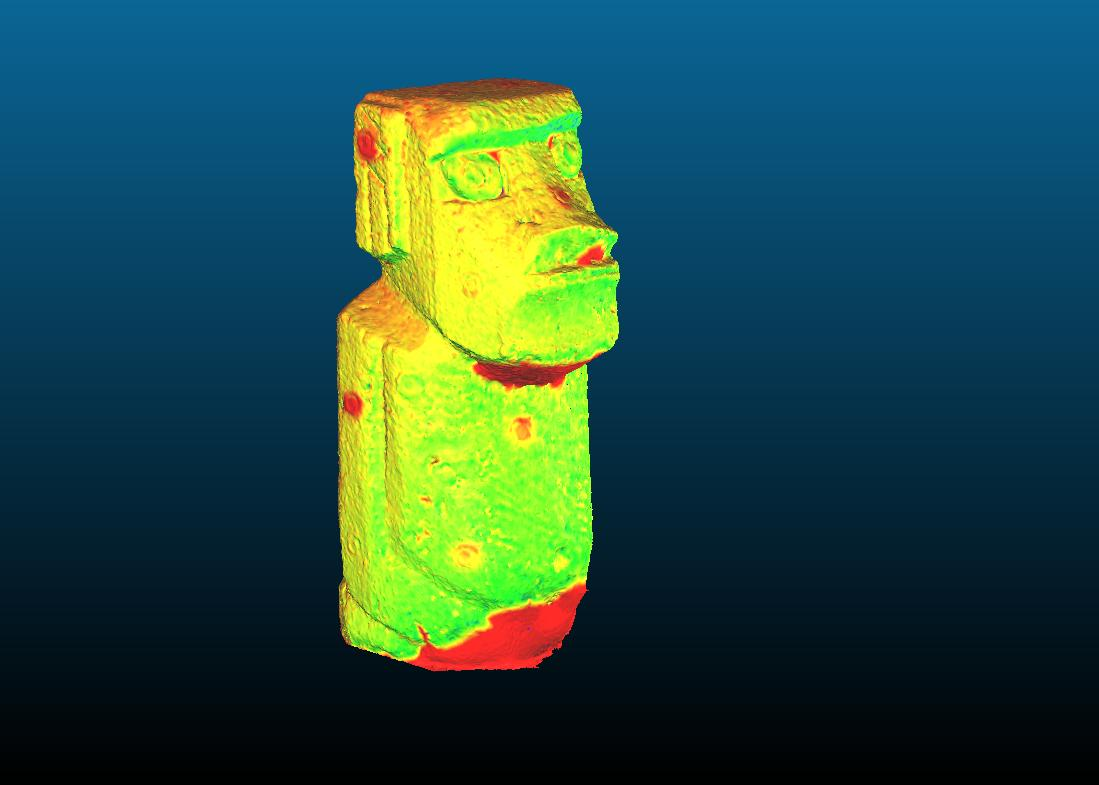
\includegraphics[width=0.8\textwidth]{img/moai_fehler.jpg}
    \caption{Differenzbild des Moai (rot: Fehler größer 0,5 mm)}
    \label{img:differenz_moai}
\end{figure}
\todo{Moai vorher erwähnen im Text}

\begin{table}
    \centering
    \caption{Ergebnisse der Genauigkeitsüberprüfung}
    \label{tab:vergleich_erg}
    \begin{tabular}{l|r|r|r}
        \toprule
                   & Durchschnittlicher & Mittlerer & Maximaler \\
                   & Fehler             & Fehler    & Fehler    \\
        %\midrule
        %Gesamt     & 0,37~mm            & 1,09~mm   & 11,6~mm   \\  % Oberflächenmodell alt
        %gefiltert  & 0,20~mm            & 0,72~mm   & 1,9~mm    \\
        \midrule
        Punktwolke & 0,04~mm            & 0,21~mm   & 3,3~mm    \\  % Vertices neu
        \midrule
        Nikon D90  & 0,27~mm            & 0,19~mm   & 1,2~mm    \\
        \bottomrule
    \end{tabular}
\end{table}


\section{Nutzung eines Drehtellers}
\label{s:drehteller}
Statt die reelle Zahl der Kameras zu erhöhen, kann auch ein Drehteller genutzt werden, sodass jede Kamera mehr als ein Bild zur Erfassung des Objektes liefert.
\todo{<> Evaluation Kameraanzahl}

\subsection{Durchführung}
Hierzu wurde ein einfacher manueller Drehteller genutzt (IKEA SNUDDA). Dieser wurde mit Passpunkten beklebt und weißt ansonsten eine texturreiche Naturholzoberfläche auf (siehe \autoref{img:drehteller_moai}). Die Daten wurden in Metashape weiterverarbeitet und die einzelnen Aufnahmeschritte über die Passpunkte und die Punktwolke zusammengerechnet. Die Ergebnisse wurden mit denen des Streifenprojektionssystems und den Aufnahmen ohne Drehteller verglichen.

\begin{figure}
    \centering
    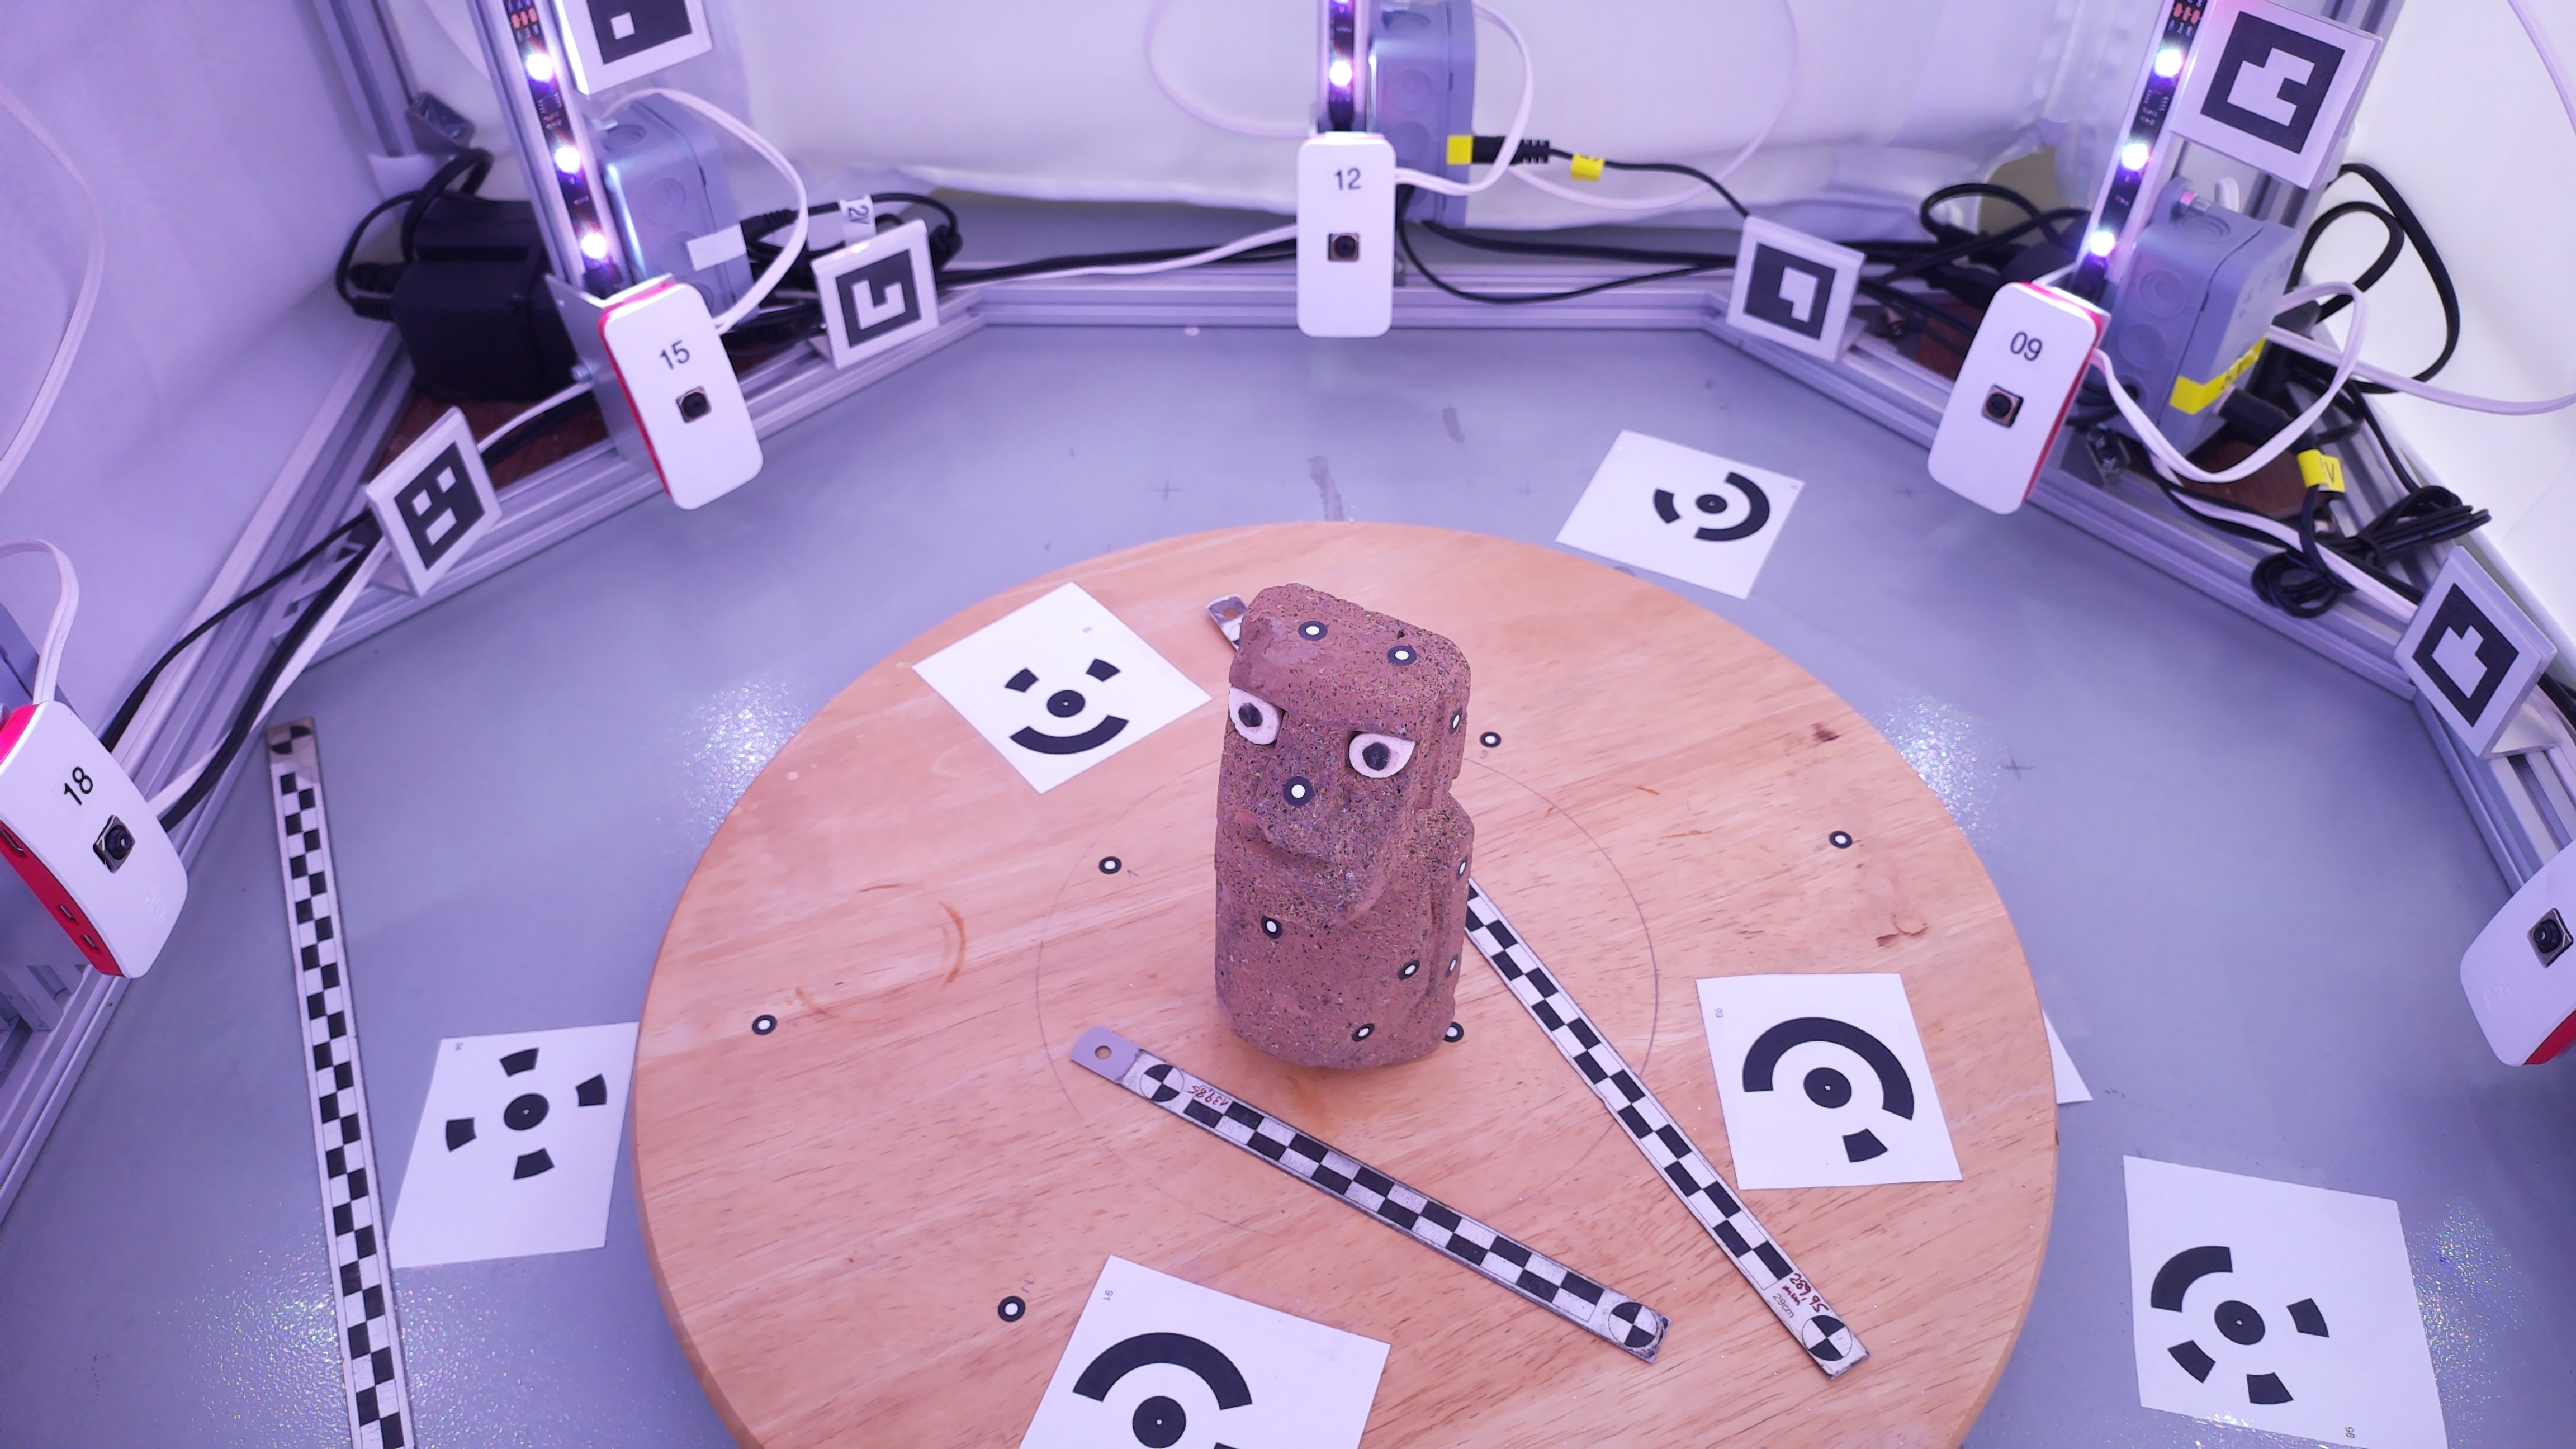
\includegraphics[width=0.8\textwidth]{img/drehteller_moai.jpg}
    \caption{Drehteller mit Moai-Figur im Prototypen (aufgenommen von einem der verbauten Raspberry Camera Module 3)}
    \label{img:drehteller_moai}
\end{figure}

\subsection{Ergebnisse}

In \autoref{img:drehteller_moai_fehler} ist das Differenzbild des Moai zu sehen. Es zeigt sich, dass die Genauigkeit des Modells mit Drehteller deutlich besser ist, als die des Modells ohne Drehteller (\autoref{img:differenz_moai}). Auch ist die visuelle Vollständigkeit deutlich höher, die nach unten gerichteten Flächen sind auch erfasst und passen gut zu dem Modell des Streifenprojektionssystems. Die Anzahl der Punkte hat sich nicht relevant verändert -- im Vergleich zu dem vollständigen Modell der Spiegelreflexkamera zeigt sich, dass über die Punktanzahl selbst keine sinnvollen Aussagen zur Abdeckung getroffen werden können.

Der geringe durchschnittliche Fehler ist auf die automatische Anpassung des Maßstabes zurückzuführen.

Die Ergebnisse sind in \autoref{tab:vergleich_drehteller} zusammengefasst.

\begin{table}
    \centering
    \caption{Ergebnisse der unter Anpassung des Maßstabes durchgeführten Genauigkeitsüberprüfung}
    \label{tab:vergleich_drehteller}
    \begin{tabular}{l|r|r|r|r}
        \toprule
                        & Durchschnittlicher & Mittlerer & Maximaler & Punktanzahl \\
                        & Fehler             & Fehler    & Fehler    &             \\
        \midrule
        ohne Drehteller & - 0,03~mm          & 0,22~mm   & 2,0~mm    & 3,3 Mio     \\
        mit Drehteller  & - 0,03~mm          & 0,15~mm   & 1,6~mm    & 3,4 Mio     \\
        Nikon D90       & 0,03~mm            & 0,17~mm   & 1,2~mm    & 0,05 Mio    \\
        \bottomrule
    \end{tabular}
\end{table}

\begin{figure}
    \centering
    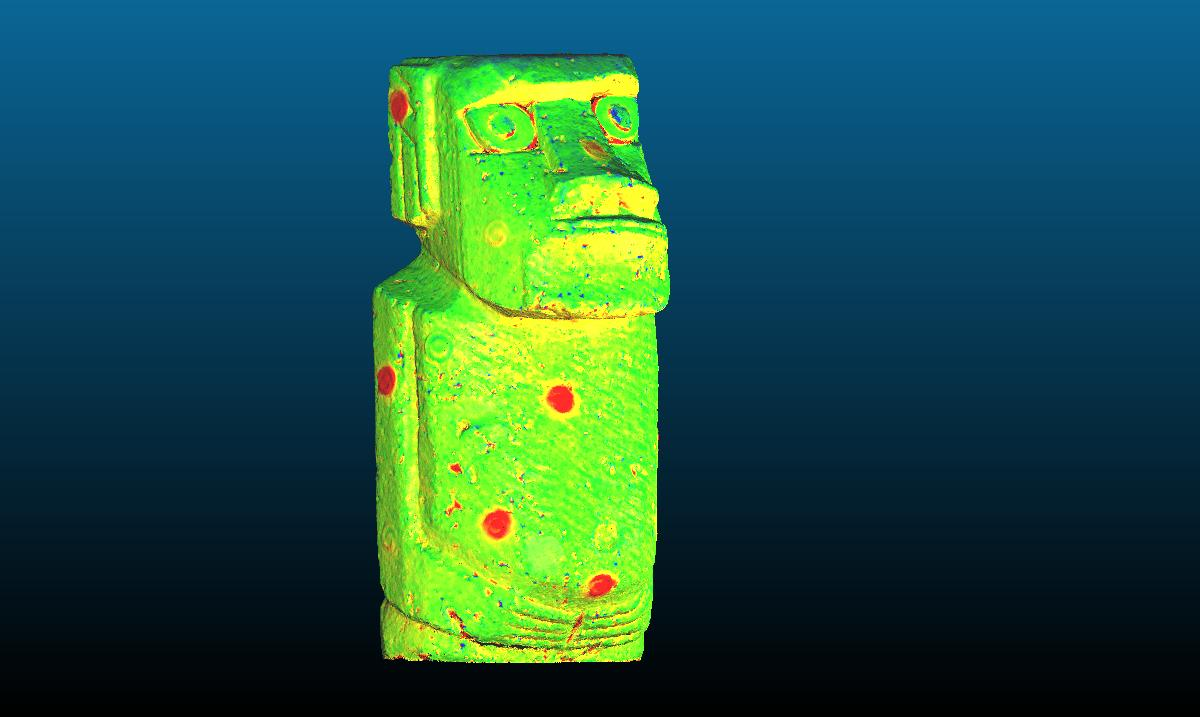
\includegraphics[width=0.8\textwidth]{img/moai_fehler_drehteller.jpg}
    \caption{Differenzbild des Moai (rot: Fehler größer 0,5 mm)}
    \label{img:drehteller_moai_fehler}
\end{figure}



\section{Evaluation der Kameraanzahl}
\label{s:kameraanzahl}
\todo{ggf. Reihenfolge mit Drehteller tauschen, gesucht: unterste Grenze, Definition?}
Die Kameras machen einen großen Teil des (Kosten-)Aufwandes zur Realisierung des Projektes aus. Es soll daher in diesem Schritt geprüft werden, ob die Anzahl der Kameras auch reduziert werden kann. Entsprechend \autoref{s:drehteller} wird auch der Einsatz des Drehtellers statt mehr Kameras geprüft.

\subsection{Durchführung}
Um abzuschätzen, wie viele Kameras für eine gute Genauigkeit notwendig sind, wurden verschiedene Konfigurationen getestet. Dazu wurde der Moai aus \autoref{s:genauigkeitsueberpruefung} verwendet und in Agisoft Metashape verschiedene Kameras deaktiviert und das 3D-Modell neu berechnet. Die Ergebnisse wurden wieder mit dem Streifenprojektionssystem verglichen. Als weiterer Parameter wurde die Abdeckung der Objektoberfläche mit Punkten bewertet. Dazu wurden die Punktwolken auf diejenigen gefiltert, die weniger als einen Millimeter vom Modell des Streifenprojektionssystems entfernt waren, auf eine Punktdichte von 1~mm Punktabstand reduziert und die Anzahl der Punkte gezählt. Darüber hinaus wurde die Anzahl der Punkte nur nach der Ausdünnung bestimmt (ohne Abstandsfilter) und mit der Anzahl mit Abstandsfilter in Beziehung gesetzt.

Als Ausgleich für fehlenden Kameras wurde auch nochmal der Drehteller aus der vorherigen Untersuchung verwendet und geprüft, wie viele Kameras durch den Drehteller ersetzt werden können.

\subsection{Ergebnisse}
Wie zu erwarten nahm die Abdeckung und die Qualität der Punktwolke ab, je weniger Kameras verwendet wurden. Bei einer Aufnahme mit allen 24 Kameras wurde die Oberfläche (ohne Boden) zu 93 \% abgedeckt. Bei einer Aufnahme mit 18 Kameras waren es nur noch 68 \% und bei 12 Kameras 54 \%.  Schon bei 18 Kameras war der Moai kaum mehr zu erkennen, bei 12 war die Erkennbarkeit nicht mehr gegeben. Die Anzahl der Kameras scheint also für dieses Objekt angebracht zu sein, sofern kein Drehteller genutzt wird.

Unter Nutzung des Drehtellers mit einer Drehung um 1/8 konnten sogar mit nur der Hälfte der Kamera ein ähnliches bzw. sogar minimal besseres Ergebnis erzielt werden, als bei der einfachen Aufnahme mit 24 Kameras. Bei der Verwendung von nur 6 Kameras in einer Ebene, so wie es bei der Planung des Rahmens auch einmal angedacht war, brachte auch die Verwendung des Drehtellers mit 4 Positionen kein brauchbares Ergebnis im direkten Anlauf. Erst durch manuelles mehrfaches Verarbeiten der Daten und die Nutzung weiterer Passpunkte konnte die Genauigkeit und Abdeckung auf ein ähnliches Niveau wie bei 12 Kameras und zwei Aufnahmen gebracht werden - dafür aber mit einem deutlich höheren personellen und technischen Aufwand.
\todo{Bilder, Tabelle, Vergleiche}

\section{Zusammenfassung}
Das System erreichte die vorgesehene Genauigkeit. Die Anzahl der Kameras war gut und für die meisten getesteten Objekte ausreichend. Der Einsatz eines Drehtellers kann die Anzahl der Kameras reduzieren, jedoch ist die Verarbeitung der Daten deutlich aufwändiger. Der Einsatz des Drehtellers zur weiteren Genauigkeitssteigerung ist aber durchaus sinnvoll, wenn die Anzahl der Kameras nicht erhöht werden kann oder soll.
\todo{weiter}

\biblio
\end{document}